\chapter{연산자, 관측량, 파울리 행렬}

좋은 표기법은 장식이 아니다. 추상 벡터와 복소수로 이루어진 학문에서, 기호를 일일이 말로 바꾸지 않고도 다룰 수 있게 해 주는 표기법은 계산의 일부다. 디랙의 브라--켓 표기법이 바로 이런 점에서 유용하다. 성분과 행렬로 계산하면서도 상태 공간의 기하학적 구조를 드러내 주기 때문이다.

당장 할 일은 수학적이다. 선형 연산자를 도입하고, 연산자가 켓뿐 아니라 브라에도 어떻게 작용하는지 알아본 다음, 에르미트 연산자라 불리는 특별한 부류를 살펴보겠다. 그런 뒤에야 \emph{관측량}, \emph{측정 결과}, \emph{확률}이라는 물리적 용어를 연결한다. 그 결과 세 가지 스핀 관측량이 외워야 할 대상으로 주어지는 대신 파울리 행렬로 나타난다.

\section{정규직교 기저와 성분}

상태들은 복소 선형 벡터 공간을 이룬다. 이 공간의 켓 벡터는 서로 더할 수 있고 복소수를 곱할 수 있다. 모든 켓 \(\ket{A}\)에는 켤레 쌍대 연산으로 얻는 브라 \(\bra{A}\)가 대응한다. 기저는 유일하지 않지만, 일단 기저를 정하면 모든 벡터를 그 기저에 대한 성분으로 나타낼 수 있다.

\[
\bigl\{\ket{1},\ket{2},\ldots,\ket{N}\bigr\}
\]
을 정규직교 기저라고 하자. 직교성과 정규화는 다음과 같이 요약된다.
\begin{equation}
\braket{j}{i}=\delta_{ji}.
\label{eq:orthonormal-basis}
\end{equation}
여기서 \(\delta_{ji}\)는 \(j=i\)일 때 1이고, 그렇지 않으면 0이다. 차원 \(N\)은 공간에서 서로 직교하는 방향을 몇 개까지 둘 수 있는지를 나타내는 최댓값이다. 완비 정규직교 기저에는 정확히 그만큼의 벡터가 들어 있다.

임의의 켓을 다음과 같이 전개하자.
\begin{equation}
\ket{A}=\sum_i \alpha_i\ket{i}.
\label{eq:ket-expansion}
\end{equation}
계수는 특별한 것이 아니다. 왼쪽에서 \(\bra{j}\)를 곱하면
\begin{align}
\braket{j}{A}
 &=\sum_i\alpha_i\braket{j}{i} \\
 &=\sum_i\alpha_i\delta_{ji}
 =\alpha_j.
\end{align}
따라서
\begin{equation}
\alpha_i=\braket{i}{A}.
\label{eq:components-inner-products}
\end{equation}
\(i\)번째 성분은 \(\ket{A}\)을 \(i\)번째 기저 방향으로 사영한 값이다.

식~\eqref{eq:components-inner-products}을 식~\eqref{eq:ket-expansion}에 대입하면 특히 유용한 다음 형태를 얻는다.
\begin{equation}
\ket{A}=\sum_i\ket{i}\braket{i}{A}.
\label{eq:ket-completeness-action}
\end{equation}
이 합은 벡터에 아무 변화도 주지 않는다. 벡터를 기저 방향들로 분해한 뒤 다시 합쳤을 뿐이다. 이 연산은 앞으로 거듭 사용하게 된다. 보통 이를 \emph{완비 상태 집합의 삽입}이라고 하는데, 그 이유는
\begin{equation}
\sum_i\ket{i}\bra{i}=\mathbf 1.
\label{eq:resolution-identity}
\end{equation}

이에 대응하는 브라 전개는 다음과 같다.
\begin{equation}
\bra{A}=\sum_i\braket{A}{i}\bra{i}
       =\sum_i\alpha_i^*\bra{i}.
\label{eq:bra-expansion}
\end{equation}
\(\alpha_i\)의 복소켤레는 반드시 필요하다. 켓을 브라로 바꾸면 모든 수치 계수가 켤레복소수가 된다.

\begin{figure}[htbp]
\centering
\includegraphics[width=0.82\textwidth]{lecture_03_figure_04.png}
\caption{기저를 살펴본 뒤 적은 선형 연산자의 두 정의 규칙.}
\lectureframe{00:12:44}
\end{figure}

\section{기계로 보는 선형 연산자}

선형 연산자 \(M\)는 입력 켓을 유일한 출력 켓으로 보내는 규칙이다. 존 휠러가 제안한 유용한 그림은 입력 포트와 출력 포트가 있는 기계다. \(\ket{A}\)를 넣고 바퀴를 돌리면 \(M\ket{A}\)를 얻는다. 입력이 정해지면 출력도 정해진다. 하지만 역방향은 유일하지 않을 수 있다. 두 입력이 같은 출력을 만들 수도 있고, 역연산 기계가 존재하지 않을 수도 있다.

\emph{선형}이라는 말에는 두 가지 규칙이 담겨 있다. 복소수 \(z\)에 대해
\begin{align}
M\bigl(z\ket{A}\bigr)&=z\,M\ket{A}, \label{eq:operator-homogeneous}\\
M\bigl(\ket{A}+\ket{B}\bigr)&=M\ket{A}+M\ket{B}.
\label{eq:operator-additive}
\end{align}
스칼라는 바뀌지 않은 채 기계를 통과하고, 합은 각 항을 따로 처리할 수 있다. 이 규칙은 임의의 유한한 복소 선형 결합에도 선형성이 성립함을 뜻한다.

같은 생각은 보통의 3차원 벡터에도 적용된다. 양자역학이 선형 사상을 새로 만들어 내는 것은 아니다. 상태 공간이 추상적이고 복소수로 이루어져 있으며, 측정 가능한 물리량을 이런 사상들의 특별한 부류로 나타내기 때문에 선형 사상이 필수적이다.

\section{연산자에서 행렬로}

기계가 \(\ket{A}\)를 \(\ket{B}\)로 보낸다고 하자.
\begin{equation}
M\ket{A}=\ket{B}.
\label{eq:operator-action}
\end{equation}
입력과 출력에 같은 정규직교 기저를 택하고 다음과 같이 쓰자.
\[
\ket{A}=\sum_j\alpha_j\ket{j},
\qquad
\ket{B}=\sum_i\beta_i\ket{i}.
\]
\(i\)번째 출력 성분을 구하려면 식~\eqref{eq:operator-action}에 \(\bra{i}\)를 곱해 사영한다.
\begin{equation}
\bra{i}M\ket{A}=\braket{i}{B}=\beta_i.
\end{equation}
이제 \(\ket{A}\)의 전개를 대입하면
\begin{align}
\bra{i}M\ket{A}
 &=\sum_j\bra{i}M\ket{j}\braket{j}{A}\\
 &=\sum_j\bra{i}M\ket{j}\alpha_j
 =\beta_i.
\end{align}
다음 수들
\begin{equation}
m_{ij}\equiv\bra{i}M\ket{j}
\label{eq:matrix-elements}
\end{equation}
은 선택한 기저에서 \(M\)의 \emph{행렬 원소}다. 따라서
\begin{equation}
\boxed{\sum_jm_{ij}\alpha_j=\beta_i.}
\label{eq:component-action}
\end{equation}

\begin{figure}[htbp]
\centering
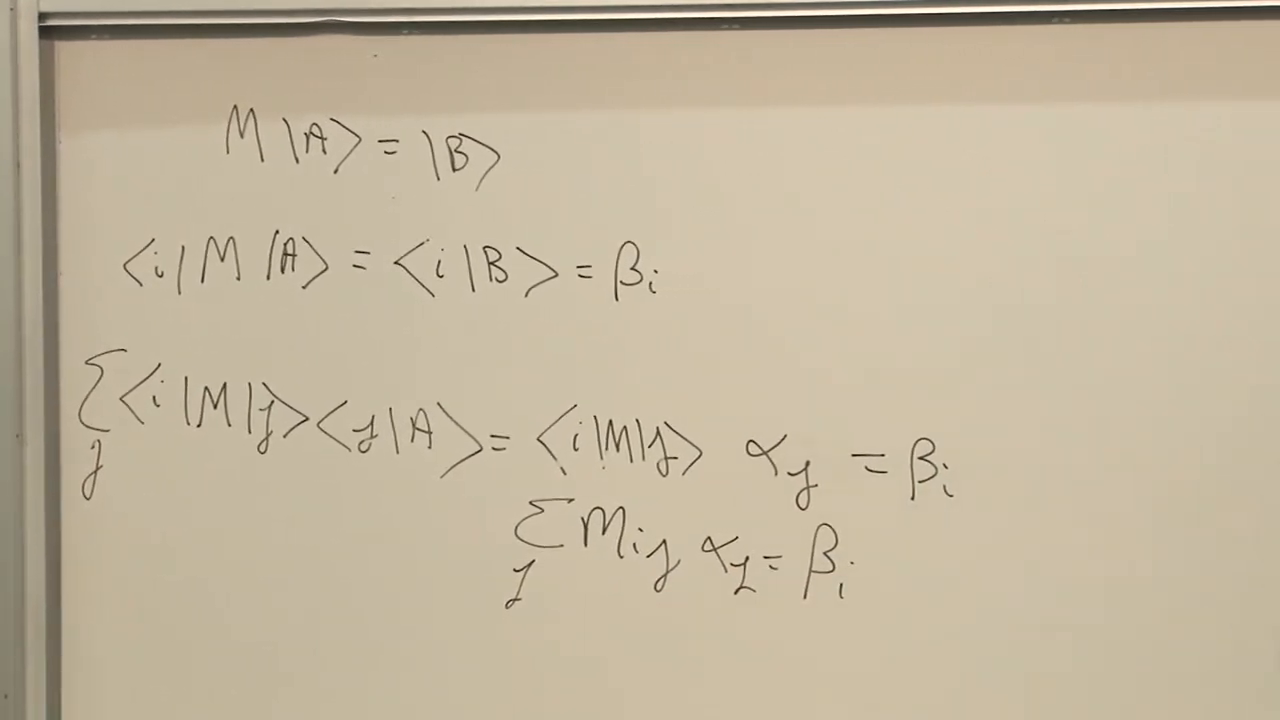
\includegraphics[width=0.84\textwidth]{lecture_03_figure_02.png}
\caption{추상 방정식 \(M\ket{A}=\ket{B}\)에 사영과 분해를 적용해 성분 규칙 \(\sum_jm_{ij}\alpha_j=\beta_i\)을 얻는다.}
\lectureframe{00:18:30}
\end{figure}

공간의 차원이 \(N\)이면 \(m_{ij}\)은 모두 \(N^2\)개이며, 이들은 \(N\times N\) 정사각 행렬을 이룬다. 식~\eqref{eq:component-action}은 정확히 다음과 같다.
\begin{equation}
\begin{pmatrix}
m_{11}&m_{12}&\cdots&m_{1N}\\
m_{21}&m_{22}&\cdots&m_{2N}\\
\vdots&\vdots&\ddots&\vdots\\
m_{N1}&m_{N2}&\cdots&m_{NN}
\end{pmatrix}
\begin{pmatrix}
\alpha_1\\
\alpha_2\\
\vdots\\
\alpha_N
\end{pmatrix}
=
\begin{pmatrix}
\beta_1\\
\beta_2\\
\vdots\\
\beta_N
\end{pmatrix}.
\label{eq:matrix-vector-action}
\end{equation}
\(\beta_1\)를 얻으려면 첫째 행에 입력 열벡터를 곱해 더하면 된다. \(\beta_2\)를 구할 때는 둘째 행을 사용하고, 이런 식으로 이어 간다. 이 행렬은 휠러의 기계를 구체적으로 나타낸 것이다.

\begin{figure}[htbp]
\centering
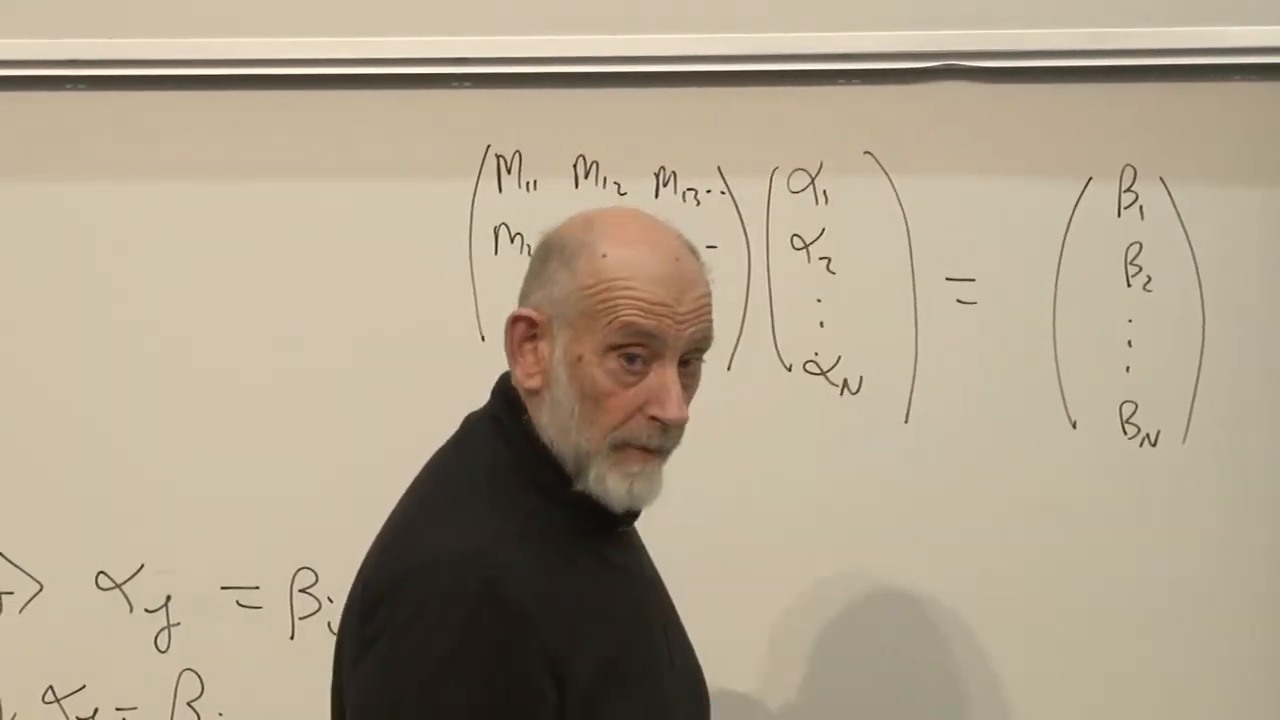
\includegraphics[width=0.84\textwidth]{lecture_03_figure_03.png}
\caption{입력 계수 열벡터에 정사각 행렬을 곱하는 형태로 나타낸 동일한 연산자 작용.}
\lectureframe{00:20:01}
\end{figure}

계산 절차를 얻은 대신 기하학적 구조가 눈에 덜 보이게 되었다. 추상적 진술 \(M\ket{A}=\ket{B}\)은 좌표에 의존하지 않는다. 반면 구체적인 원소 \(m_{ij}\), \(\alpha_j\), \(\beta_i\)은 선택한 기저에 따라 달라진다. 다른 정규직교 기저를 택하면 세 배열 모두 달라지지만, 그 바탕에 있는 사상과 물리적 예측은 변하지 않는다.

\begin{classroomqa}\audiencequestion{기저의 선택에 따라 문제를 풀 수 있는지가 달라질 수 있나요?}\lecturerresponse{해답을 쉽게 알아볼 수 있는지는 달라질 수 있습니다. 기저를 잘 고르면 연산자가 대각화되어 계산이 거의 바로 끝날 수도 있고, 잘못 고른 기저에서는 구조가 불편한 대수식 아래 가려질 수 있습니다. 하지만 기저 선택이 실험 결과를 바꿀 수는 없습니다. 두 기저를 사용한 계산에서 서로 다른 물리적 답이 나온다면 계산이 틀린 것입니다.}\end{classroomqa}

\section{브라, 켓, 반선형성}

\begin{classroomqa}\audiencequestion{선형 연산자가 켓을 브라로, 또는 브라를 켓으로 바꿀 수 있나요?}\lecturerresponse{방금 정의한 보통의 선형 연산자는 그럴 수 없습니다. 이 연산자는 켓을 켓으로 보내며 복소 스칼라는 바뀌지 않은 채 통과합니다. 켓과 브라를 서로 바꾸는 연산은 계수도 켤레복소수로 바꾸므로 다른 부류에 속합니다.}\end{classroomqa}

고정된 복소수를 곱하는 것은 간단한 선형 연산자다. 복소켤레를 취하는 연산은 선형이 아니다. \(K\)가 켤레복소수 연산을 뜻한다면
\[
K\bigl(z\ket{A}\bigr)=z^*K\ket{A},
\]
이지 \(zK\ket{A}\)가 아니다. 이런 사상을 \emph{반선형}이라고 한다. 이 이름은 선형의 반대라는 뜻이 아니라 스칼라의 켤레복소수를 취한다는 뜻이다. 반입자와의 더 깊은 연관성은 여기서 다루지 않는다.

그래도 선형 연산자가 브라에 작용하도록 할 수 있다. 약속에 따라 연산자를 오른쪽에 쓴다.
\begin{equation}
\bra{A}M.
\end{equation}
행렬 원소에 괄호를 어디에 둘지 모호하지 않도록 이 작용을 정의한다.
\begin{equation}
\bra{A}\bigl(M\ket{B}\bigr)
=
\bigl(\bra{A}M\bigr)\ket{B}
\equiv
\bra{A}M\ket{B}.
\label{eq:bracket-independence}
\end{equation}

이 정의가 가능한 이유를 보려면 두 벡터를 모두 전개하면 된다.
\begin{align}
\bra{A}M\ket{B}
 &=\left(\sum_i\alpha_i^*\bra{i}\right)
   M
   \left(\sum_j\beta_j\ket{j}\right)\\
 &=\sum_{ij}\alpha_i^*m_{ij}\beta_j.
\label{eq:matrix-element-double-sum}
\end{align}
이 식은 보통의 이중 합이다. 먼저 \(j\)에 대해 합하고 \(M\)가 켓에 작용한다고 볼 수도 있고, 먼저 \(i\)에 대해 합하고 연산자가 브라에 작용한다고 볼 수도 있다. 어느 쪽이든 결과는 같다. 불필요한 괄호를 없앨 수 있도록 표기법을 바로 이렇게 정한 것이다.

\section{대거 연산}

브라 쪽에는 이와 별개인 또 다른 질문이 있다. 다음과 같다고 하자.
\[
M\ket{A}=\ket{B}.
\]
이에 대응하는 브라 \(\bra{A}\)를 \(\bra{B}\)로 바꾸는 연산자는 무엇일까? 일반적으로 \(M\) 자체는 아니다. \(M\)가 복소수 \(z\)를 곱하는 연산자라면, 켓 방정식은 \(\ket{B}=z\ket{A}\)이지만 브라 방정식은 \(\bra{B}=z^*\bra{A}\)이다.

필요한 연산자를 \(M^\dagger\)로 쓰며, 이는 \(M\)\emph{에르미트 켤레}라고 한다. 다음과 같이 정의한다.
\begin{equation}
M\ket{A}=\ket{B}
\quad\Longleftrightarrow\quad
\bra{A}M^\dagger=\bra{B}.
\label{eq:dagger-definition}
\end{equation}
대거는 복소켤레 연산자에 대응하는 연산자다.

행렬에 대한 규칙은 바로 유도할 수 있다. 다음과 같이 두자.
\[
M\ket{i}=\ket{i'}.
\]
그러면
\[
m_{ji}=\bra{j}M\ket{i}=\braket{j}{i'}.
\]
대거를 취한 브라 관계는 \(\bra{i}M^\dagger=\bra{i'}\)이므로
\[
(m^\dagger)_{ij}
=\bra{i}M^\dagger\ket{j}
=\braket{i'}{j}.
\]
내적의 순서를 뒤집으면 복소켤레를 취하게 된다.
\[
\braket{i'}{j}=\braket{j}{i'}^*.
\]
따라서
\begin{equation}
\boxed{(m^\dagger)_{ij}=m_{ji}^*.}
\label{eq:dagger-matrix-elements}
\end{equation}

\begin{figure}[htbp]
\centering
\includegraphics[width=0.84\textwidth]{lecture_03_figure_05.png}
\caption{에르미트 켤레에 대한 완성된 판서식 관계: 첨자를 서로 바꾸고 복소켤레를 취한다.}
\lectureframe{00:42:23}
\end{figure}

행렬로 표현하면 먼저 전치한 다음 복소켤레를 취한다.
\begin{equation}
\begin{pmatrix}
a&b\\
c&d
\end{pmatrix}^{\!\dagger}
=
\begin{pmatrix}
a^*&c^*\\
b^*&d^*
\end{pmatrix}.
\label{eq:dagger-two-by-two}
\end{equation}
전치는 주대각선을 기준으로 원소들을 서로 바꾸고, 켤레복소수 연산은 모든 \(i\)를 \(-i\)로 바꾼다. 예를 들면
\begin{equation}
\begin{pmatrix}
2&6+7i\\
4-i&9+i
\end{pmatrix}^{\!\dagger}
=
\begin{pmatrix}
2&4+i\\
6-7i&9-i
\end{pmatrix}.
\label{eq:dagger-numerical-example}
\end{equation}
대각 원소는 제자리에 남아 켤레복소수로 바뀌고, 두 비대각 원소는 자리를 서로 바꾸면서 켤레복소수로 바뀐다.

\section{에르미트 연산자}

복소수가 자신의 켤레복소수와 같을 때, 그리고 그때에만 그 수는 실수다. 연산자에도 바로 대응하는 성질이 있다.

\begin{definition}정의\(M\) 연산자 \emph{에르미트} 연산자는 다음을 만족한다.
\begin{equation}
M=M^\dagger.
\label{eq:hermitian-definition}
\end{equation}
동치로, 모든 정규직교 기저에서
\begin{equation}
m_{ij}=m_{ji}^*.
\label{eq:hermitian-components}
\end{equation}
을 만족한다.\end{definition}

식~\eqref{eq:hermitian-components}에서 \(i=j\)으로 두면
\[
m_{ii}=m_{ii}^*,
\]
이므로 모든 대각 원소는 실수다. 대각선 밖의 원소들은 켤레복소수로 서로 대응한다. 한 원소가 \(4-i\)이면, 대칭 위치의 원소는 \(4+i\)이다. 한 원소가 실수 \(5\)이면 그 짝도 실수다.

\begin{figure}[htbp]
\centering
\includegraphics[width=0.78\textwidth]{lecture_03_figure_06.png}
\caption{완성된 에르미트 행렬의 예: 대각선에는 실수 원소가 있고, 대각선을 중심으로 복소켤레 쌍이 서로 대응한다.}
\lectureframe{00:45:43}
\end{figure}

에르미트 연산자는 측정 가능한 물리량을 나타내게 되므로 중요하다. 그 연결을 설명하기에 앞서, 에르미트 연산자의 고유 방향을 이해해야 한다.

\section{고유벡터와 고유 방향}

고유벡터를 처음 접하면 이 부분이 주변의 물리 내용보다 빠르게 진행된다고 느낄 수 있다. 이 내용은 새로운 물리적 가설이 아니라 표준 선형대수다. 익숙하지 않다면 정의를 차분히 복습한 뒤 논의를 이어 가는 편이 좋다.

일반적인 연산자는 벡터의 방향을 바꾼다. 예를 들어 보통의 3차원 공간에서 회전을 하면 거의 모든 벡터의 방향이 바뀐다. 회전축만은 예외다. 그 축을 따라 놓인 벡터는 회전 후에도 같은 방향을 가리킨다. 이것이 고유벡터의 전형적인 예다.

실수 2차원 평면에서의 자명하지 않은 회전은 정반대의 가능성을 보여 준다. 실수 배를 허용하더라도 변하지 않는 실수 방향이 없다. 따라서 제한된 실수 공간에서 일반적인 연산자는 실수 고유벡터를 갖지 않을 수 있다. 양자역학에서 쓰는 복소 상태 공간의 에르미트 연산자는 훨씬 강한 성질을 갖는다.

\(M\)의 고유벡터는 다음을 만족한다.
\begin{equation}
M\ket{i}=\lambda_i\ket{i}.
\label{eq:eigenvalue-equation}
\end{equation}
수 \(\lambda_i\)는 그 고윳값이다. 고유벡터는 연산자에 속한다. 방향을 보존하는 사상이 무엇인지 지정하지 않은 채 고유벡터를 말할 수는 없다.

그 크기와 위상은 식~\eqref{eq:eigenvalue-equation}으로 정해지지 않는다. 영이 아닌 모든 복소수 \(z\)에 대해
\[
M\bigl(z\ket{i}\bigr)
=zM\ket{i}
=\lambda_i\bigl(z\ket{i}\bigr).
\]
따라서 \emph{고유방향}이라고 하는 편이 더 정확하다. \(\ket{i}\)의 영이 아닌 모든 배수는 같은 방향을 나타내며 같은 고유값을 갖는다. 보통은 그중 정규화된 상태를 하나 택한다.

핵심적인 스펙트럼 정리는 다음과 같다. \(N\)차원 복소 벡터 공간 위의 에르미트 연산자는 \(N\)개의 고유벡터로 이루어진 완비 정규직교 기저를 갖는다. 이 진술의 두 부분은 대수 계산을 거의 하지 않고도 확인할 수 있다.

\subsection{에르미트 연산자의 고윳값은 실수}

\(M=M^\dagger\)이라고 가정하자. 그리고
\[
M\ket{i}=\lambda_i\ket{i}.
\]
식 전체의 에르미트 켤레를 취하면
\begin{equation}
\bra{i}M^\dagger=\lambda_i^*\bra{i}.
\label{eq:eigen-bra-equation}
\end{equation}
\(M^\dagger=M\)이므로, 켓 방정식의 왼쪽에 \(\bra{i}\)을 곱하고 브라 방정식의 오른쪽에 \(\ket{i}\)을 곱하면
\begin{align}
\bra{i}M\ket{i}&=\lambda_i\braket{i}{i},\\
\bra{i}M\ket{i}&=\lambda_i^*\braket{i}{i}.
\end{align}
두 값에 같은 영이 아닌 노름이 곱해지므로
\begin{equation}
\lambda_i=\lambda_i^*.
\end{equation}
에르미트 연산자의 모든 고유값은 실수이다. 이것은 그러한 연산자가 측정 장치에 표시되는 실수를 나타낼 수 있음을 보여 주는 첫 단서다.

\subsection{서로 다른 고윳값에 대응하는 고유벡터는 직교한다}

다음과 같이 두자.
\[
M\ket{i}=\lambda_i\ket{i},
\qquad
M\ket{j}=\lambda_j\ket{j},
\]
여기서 \(M\)는 에르미트 연산자다. 둘째 식에 대거를 취한다. 고윳값이 실수라는 점은 이미 확인했다.
\[
\bra{j}M=\lambda_j\bra{j}.
\]
이제 첫째 식에는 왼쪽에서 \(\bra{j}\)를, 브라 식에는 오른쪽에서 \(\ket{i}\)를 곱하면
\begin{align}
\bra{j}M\ket{i}&=\lambda_i\braket{j}{i},\\
\bra{j}M\ket{i}&=\lambda_j\braket{j}{i}.
\end{align}
두 식을 빼면
\begin{equation}
\boxed{(\lambda_i-\lambda_j)\braket{j}{i}=0.}
\label{eq:hermitian-orthogonality}
\end{equation}
\(\lambda_i\ne\lambda_j\)이면
\[
\braket{j}{i}=0.
\]
이 되어 고유 방향들은 서로 직교한다.

\begin{figure}[htbp]
\centering
\includegraphics[width=0.82\textwidth]{lecture_03_figure_07.png}
\caption{직교성을 증명하는 결정적인 단계: 서로 다른 고유값이면 내적은 영이어야 한다.}
\lectureframe{00:59:00}
\end{figure}

두 고윳값이 같으면 식~\eqref{eq:hermitian-orthogonality}은 그 축퇴 고유공간 안에서 아무런 조건도 부과하지 않는다. 그 공간 안에서 정규직교 기저를 택할 수 있다. 이 벡터들을 나머지 고유 방향들과 합치면 스펙트럼 정리가 보장하는 완비 정규직교 고유기저가 된다.

직교성에는 물리적 의미도 있다. 두 직교 상태는 적절한 측정으로 모호함 없이 구별할 수 있다. 고윳값이 다른 고유상태들은 장치가 서로 다른 실숫값을 표시하므로 구별할 수 있어야 한다. 대수적 관계와 조작적 의미가 이미 같은 대응을 가리키고 있다.

\section{측정 공준}

이제 양자역학의 기본적인 대응 관계를 진술하기에 필요한 형식 체계를 갖췄다. 처음 접하면 낯설게 들릴 수 있다. 실제로 적용해야 비로소 의미가 구체적으로 드러나므로, 먼저 간결하게 진술한 뒤 곧바로 스핀 실험으로 돌아가자.

한 번의 측정은 실수를 산출한다. 서로 양립하는 두 실숫값을 하나의 복소수로 묶을 수는 있지만, 그 묶음에도 측정 두 번의 결과가 들어 있다. 한 검출기가 내놓는 기본적인 결과는 실수다. 따라서 에르미트 연산자가 자연스러운 후보가 된다. 에르미트 연산자의 고윳값은 실수이고, 고유벡터들은 완비 정규직교 기저를 이루기 때문이다.

\begin{enumerate}
\item \emph{측정 가능한 물리량, 즉 관측량}은 에르미트 연산자 \(M\)로 나타낸다.
\item \(M\)를 측정했을 때 얻을 수 있는 결과는 그 고윳값 \(\lambda_i\)이다.
\item \(M\)가 확정된 값 \(\lambda_i\)을 갖는 상태는 다음을 만족하는 고유상태 \(\ket{i}\)다.
\[
M\ket{i}=\lambda_i\ket{i}.
\]
\item \(\ket{A}\)가 일반적인 정규화 상태라면, \(\lambda_i\)을 얻을 확률은
\begin{equation}
P(\lambda_i\mid A)
=\left|\braket{i}{A}\right|^2
=\braket{i}{A}\braket{A}{i}.
\label{eq:born-rule}
\end{equation}
\end{enumerate}

이 목록은 편리한 출발점이지만, 반드시 최소한의 독립 공리계인 것은 아니다. 더 간결하게 정식화하면 일부 진술을 다른 진술로부터 유도할 수 있다. 대응 관계를 구분해 두면 각 항목의 물리적 역할을 더 쉽게 파악할 수 있다.

복소수 \(\braket{i}{A}\)는 \emph{확률진폭}이지 확률이 아니다. 여기에 켤레복소수를 곱하면 실수인 음이 아닌 값이 나온다. 스핀 성분의 스펙트럼에는 \(+1\)와 \(-1\), 두 값만 있다. 더 일반적인 관측량은 여러 고윳값을 가질 수 있다.

\begin{figure}[htbp]
\centering
\includegraphics[width=0.82\textwidth]{lecture_03_figure_08.png}
\caption{판서에서는 확정된 결과를 갖는 상태를 고유벡터와 연결하고, \(\lambda_i\)을 얻을 확률을 \(\ket{i}\)에 대한 사영의 제곱으로 나타낸다.}
\lectureframe{01:11:29}
\end{figure}

\begin{classroomqa}\audiencequestion{확률 규칙에서 \(P\) 옆에 쓰인 것은 정확히 무엇인가요?}\lecturerresponse{\(\lambda_i\)입니다. \(P(\lambda_i\mid A)\)는 계가 \(\ket{A}\) 상태로 준비되었을 때 \(M\)를 측정해 특정 고윳값 \(\lambda_i\)을 얻을 확률을 뜻합니다. 우변은 그 고유벡터에 대한 사영의 크기를 제곱한 값입니다.}\end{classroomqa}

\subsection{정규화와 완비성}

서로 배타적인 모든 결과의 확률을 더하면 1이어야 한다.
\begin{equation}
\sum_i\left|\braket{i}{A}\right|^2=1.
\label{eq:probability-normalization}
\end{equation}
완비 고유기저를 삽입하면
\begin{align}
\sum_i\left|\braket{i}{A}\right|^2
 &=\sum_i\braket{A}{i}\braket{i}{A}\\
 &=\bra{A}\left(\sum_i\ket{i}\bra{i}\right)\ket{A}\\
 &=\braket{A}{A}.
\end{align}
따라서 허용되는 상태 벡터는 정규화되어 있다.
\begin{equation}
\braket{A}{A}=1.
\label{eq:state-normalization}
\end{equation}
\(\ket{A}=\sum_i\alpha_i\ket{i}\)이면 같은 조건은
\begin{equation}
\sum_i\alpha_i^*\alpha_i=1.
\label{eq:component-normalization}
\end{equation}
이다. 이는 복소 성분들에 부과되는 하나의 실수 조건이다.

\begin{classroomqa}\audiencequestion{모든 확률은 양수여야 하나요?}\lecturerresponse{그렇습니다. 각 확률은 어떤 수에 그 수의 켤레복소수를 곱한 값이므로 음이 아닌 실수입니다. 정규화 조건에 따라 그런 값들을 모두 더하면 1이 됩니다.}\end{classroomqa}

또 다른 중복성이 있다. 모든 성분에 같은 위상을 곱하면
\begin{equation}
\ket{A}\longmapsto e^{i\theta}\ket{A},
\label{eq:l3-global-phase}
\end{equation}
모든 진폭에 \(e^{i\theta}\)가 곱해지지만, 각 진폭의 제곱한 크기는 변하지 않는다. 어떤 측정으로도 이 공통 위상을 알아낼 수 없다. 성분 사이의 상대 위상은 물리적 의미가 있지만, 상태 전체에 곱해지는 위상만은 중복된 표현이다.

따라서 임의의 복소 벡터를 이루는 두 실수 매개변수만으로 물리적 상태를 지정할 수는 없다. 정규화 조건이 벡터의 크기를 정하고 전체 위상은 관측할 수 없기 때문이다. 이는 이제 일반적인 확률 규칙에서 유도한, 단일 스핀에서 얻었던 것과 같은 매개변수 개수다.

\subsection{측정은 상태도 준비한다}

또 하나의 공준은 짧은 판서식으로 압축하기보다 말로 설명하는 편이 쉽다. 측정 결과가 \(\lambda_i\)이면, 그 직후 계는 그에 대응하는 고유상태 \(\ket{i}\)에 있다. 측정 장치는 결과를 기록하는 동시에, 같은 측정을 반복하면 확정된 결과를 얻을 상태를 준비한다.

\begin{classroomqa}\audiencequestion{측정이 상태를 준비한다는 내용을 다시 한번 설명해 주시겠어요?}\lecturerresponse{측정 전에는 식~\eqref{eq:born-rule}에 주어진 확률에 따라 여러 고윳값이 나올 수 있습니다. 장치가 실제로 \(\lambda_i\)을 표시하면, 계는 \(\lambda_i\)에 해당하는 고유상태로 남습니다. 따라서 같은 관측량을 바로 한 번 더 측정하면 같은 값이 나옵니다.}\end{classroomqa}

\begin{classroomqa}\audiencequestion{이 원리만으로 상태의 시간에 따른 변화를 알 수 있나요?}\lecturerresponse{아직은 아닙니다. 상태가 무엇인지, 관측량을 어떻게 나타내는지, 측정이 무엇을 하는지는 정했습니다. 시간에 따른 변화를 지배하는 법칙은 추가적인 구조이며 나중에 도입하겠습니다. 운동 방정식을 쓰기 전에 고전적인 위상 공간부터 정의하는 것과 비슷합니다.}\end{classroomqa}

\begin{classroomqa}\audiencequestion{앞서 기울어진 축을 따른 평균 스핀에 \(\cos\theta\)가 들어갔습니다. 이제 새로 배운 진폭 제곱 규칙에 따르면 그 값은 \(\cos^2\theta\)이 되어야 하나요?}\lecturerresponse{확률과 평균은 서로 다른 양입니다. 평균은 \(+1\)와 \(-1\) 결과가 나올 확률에 각각 그 부호를 반영해 합한 값입니다. 임의의 방향에 대한 스피너를 구성하면, 제곱한 진폭에서 앞서 얻은 코사인 평균이 나옵니다. 이 계산은 다음 적용 사례로 다룰 내용이지, 이전 공식을 바꾸어 추측할 내용이 아닙니다.}\end{classroomqa}

\section{첫 번째 적용 사례, 스핀}

측정 가능한 세 스핀 성분은 에르미트 연산자
\[
\sigma_x,\qquad \sigma_y,\qquad \sigma_z.
\]
로 나타낸다. 분석기 실험을 통해 가능한 값과 확정된 값을 갖는 상태도 이미 알게 되었다.
\[
\begin{array}{c|c|c}
\text{observable}&\text{eigenvalue }+1&\text{eigenvalue }-1\\ \hline
\sigma_z&\ket{u}&\ket{d}\\
\sigma_x&\ket{r}&\ket{l}\\
\sigma_y&\ket{\mathrm{in}}&\ket{\mathrm{out}}
\end{array}
\]
이 정보만으로 연산자들을 행렬로 재구성할 수 있다.

\subsection{고유기저에서의 z 성분}

업--다운 기저를 택하자. 확정된 \(z\)-스핀은 다음을 뜻한다.
\begin{equation}
\sigma_z\ket{u}=+\ket{u},
\qquad
\sigma_z\ket{d}=-\ket{d}.
\label{eq:sigma-z-eigenvectors}
\end{equation}
두 고윳값이 다르므로 에르미트성에 따라 \(\braket{u}{d}=0\)이다.

행렬 원소 네 개를 계산하면
\begin{align}
\bra{u}\sigma_z\ket{u}&=+1,&
\bra{u}\sigma_z\ket{d}&=-\braket{u}{d}=0,\\
\bra{d}\sigma_z\ket{u}&=\braket{d}{u}=0,&
\bra{d}\sigma_z\ket{d}&=-1.
\end{align}
따라서
\begin{equation}
\boxed{
\sigma_z=
\begin{pmatrix}
1&0\\
0&-1
\end{pmatrix}_{\{u,d\}}.}
\label{eq:sigma-z}
\end{equation}
좌표 열벡터는
\[
\ket{u}\widehat{=}\begin{pmatrix}1\\0\end{pmatrix},
\qquad
\ket{d}\widehat{=}\begin{pmatrix}0\\1\end{pmatrix}.
\]
이다. 식~\eqref{eq:sigma-z}의 행렬을 곱하면 첫째 열은 그대로, 둘째 열은 부호가 바뀌어 나온다. 고윳값 방정식이 요구하는 결과와 정확히 일치한다.

\begin{figure}[htbp]
\centering
\includegraphics[width=0.82\textwidth]{lecture_03_figure_09.png}
\caption{업\(\sigma_z\) 고윳값 방정식과 업--다운 기저에서 얻은 대각 행렬.}
\lectureframe{01:26:56}
\end{figure}

\subsection{기저를 바꾸지 않고 구하는 x 성분}

라이트--레프트 기저에서는 \(\sigma_x\)가 같은 대각 형태를 갖는다. 계산은 쉽겠지만 얻는 것이 없다. 업--다운 기저를 그대로 두고 다음을 사용하자.
\begin{equation}
\sigma_x\ket{r}=+\ket{r},
\qquad
\sigma_x\ket{l}=-\ket{l}.
\label{eq:sigma-x-eigenvectors}
\end{equation}
두 기저는 다음 관계를 만족한다.
\begin{align}
\ket{r}&=\frac{\ket{u}+\ket{d}}{\sqrt2},&
\ket{l}&=\frac{\ket{u}-\ket{d}}{\sqrt2},\\
\ket{u}&=\frac{\ket{r}+\ket{l}}{\sqrt2},&
\ket{d}&=\frac{\ket{r}-\ket{l}}{\sqrt2}.
\label{eq:x-z-basis-relations}
\end{align}

먼저 왼쪽 위 대각 성분부터 살펴보자:
\begin{align}
\bra{u}\sigma_x\ket{u}
 &=\frac12(\bra{r}+\bra{l})\sigma_x(\ket{r}+\ket{l})\\
 &=\frac12(\bra{r}+\bra{l})(\ket{r}-\ket{l})\\
 &=0.
\end{align}
오른쪽 상태와 왼쪽 상태는 서로 직교 정규이므로 두 대각 항은 상쇄되고 교차 항은 사라진다. \(\ket{d}\)에 대해서도 같은 계산을 하면
\[
\bra{d}\sigma_x\ket{d}=0.
\]
이 단계에서 두 항이 영이라고 해서 연산자가 영 연산자라는 뜻은 아니다. 대각 성분이 아닌 곳을 살펴보라는 뜻이다.

첫째 행, 둘째 열의 원소는
\begin{align}
\bra{u}\sigma_x\ket{d}
 &=\frac12(\bra{r}+\bra{l})\sigma_x(\ket{r}-\ket{l})\\
 &=\frac12(\bra{r}+\bra{l})(\ket{r}+\ket{l})\\
 &=1.
\end{align}
에르미트성에 따라, 또는 직접 같은 계산을 반복하면
\[
\bra{d}\sigma_x\ket{u}=1.
\]
을 얻는다. 따라서
\begin{equation}
\boxed{
\sigma_x=
\begin{pmatrix}
0&1\\
1&0
\end{pmatrix}_{\{u,d\}}.}
\label{eq:sigma-x}
\end{equation}
같은 추상 연산자도 자신의 고유기저에서는 대각 행렬이고 \(z\)-기저에서는 대각선 밖에 원소가 있다. 이는 기저에 따른 표현의 차이가 물리적 모호성을 뜻하지 않는다는 구체적인 예다.

\subsection{y 성분과 상대 위상}

정규화된 인--아웃 규약을 다음과 같이 택하자.
\begin{equation}
\ket{\mathrm{in}}=\frac{\ket{u}+i\ket{d}}{\sqrt2},
\qquad
\ket{\mathrm{out}}=\frac{\ket{u}-i\ket{d}}{\sqrt2},
\label{eq:l3-in-out-states}
\end{equation}
여기서
\[
\sigma_y\ket{\mathrm{in}}=+\ket{\mathrm{in}},
\qquad
\sigma_y\ket{\mathrm{out}}=-\ket{\mathrm{out}}.
\]
이다. 라벨을 맞바꾸거나 \(y\)축의 방향을 반대로 하면 부호 규약은 바뀌지만, 바탕이 되는 구성은 변하지 않는다. 식~\eqref{eq:l3-in-out-states}을 사용하면 이 고유벡터와 고윳값을 갖는 유일한 에르미트 행렬은
\begin{equation}
\boxed{
\sigma_y=
\begin{pmatrix}
0&-i\\
i&0
\end{pmatrix}_{\{u,d\}}.}
\label{eq:sigma-y}
\end{equation}
이다. 다시 유도하지 않고 확인하기는 쉽다.
\begin{align}
\begin{pmatrix}0&-i\\i&0\end{pmatrix}
\frac1{\sqrt2}\begin{pmatrix}1\\i\end{pmatrix}
&=\frac1{\sqrt2}\begin{pmatrix}1\\i\end{pmatrix},\\
\begin{pmatrix}0&-i\\i&0\end{pmatrix}
\frac1{\sqrt2}\begin{pmatrix}1\\-i\end{pmatrix}
&=-\frac1{\sqrt2}\begin{pmatrix}1\\-i\end{pmatrix}.
\end{align}
\(1/\sqrt2\) 인자는 고유벡터를 정규화하지만 고유 방향에는 영향을 주지 않는다.

\begin{figure}[htbp]
\centering
\includegraphics[width=0.82\textwidth]{lecture_03_figure_10.png}
\caption{업--다운 기저에서 얻은 파울리 행렬 세 개를 모두 판서에 나타냈다.}
\lectureframe{01:38:11}
\end{figure}

\begin{classroomqa}\audiencequestion{인--아웃 벡터가 서로 직교하도록 부호 하나를 바꿔야 하나요?}\lecturerresponse{아닙니다. 빠뜨린 단계는 켓을 브라로 바꿀 때 복소켤레를 취하는 것입니다.
\[
\bra{\mathrm{in}}=\frac{\bra{u}-i\bra{d}}{\sqrt2}.
\]
따라서
\[
\begin{aligned}
\braket{\mathrm{in}}{\mathrm{out}}
&=\frac12(\bra{u}-i\bra{d})
  (\ket{u}-i\ket{d})\\
&=\frac12\bigl(1+(-i)(-i)\bigr)\\
&=0.
\end{aligned}
\]
그 켤레복소수 취하기를 잊는 것이 바로 브라--켓 표기법이 드러내려는 흔한 실수입니다.}\end{classroomqa}

다음과 같이 얻었다.
\begin{equation}
\begin{aligned}
\sigma_x&=\begin{pmatrix}0&1\\1&0\end{pmatrix},\\[0.4em]
\sigma_y&=\begin{pmatrix}0&-i\\i&0\end{pmatrix},\\[0.4em]
\sigma_z&=\begin{pmatrix}1&0\\0&-1\end{pmatrix}.
\end{aligned}
\label{eq:pauli-triple}
\end{equation}
이들은 에르미트 연산자이고, 고윳값 \(\pm1\)를 가지며, 분석기 실험에서 요구된 확정된 스핀의 고유벡터를 정확히 갖는다.

이제 다음 문제를 명확히 제시할 수 있다. 임의의 방향으로 스핀을 준비했을 때 그에 대응하는 상태를 구성하고, 제곱한 진폭을 이용해 \(\sigma_z=+1\)와 \(\sigma_z=-1\)를 얻을 확률을 계산하자. 형식 체계에는 이미 필요한 정보가 모두 들어 있으므로, 그 계산을 수행하는 것이 자연스러운 다음 단계다.
